% !TeX root = ./ms.tex
\documentclass[modern]{aastex62}

% Load the corTeX style definitions
% !TeX root = ./ms.tex
% All the packages
\usepackage{url}
\usepackage{amsmath}
\usepackage{mathtools}
\usepackage{amssymb}
\usepackage{natbib}
\usepackage{graphicx}
\usepackage{calc}
\usepackage{etoolbox}
\usepackage{xspace}
\usepackage[T1]{fontenc} % https://tex.stackexchange.com/a/166791
\usepackage{textcomp}
\usepackage{ifxetex}
\ifxetex
  \usepackage{fontspec}
  \defaultfontfeatures{Extension = .otf}
\fi
\usepackage{fontawesome}
\usepackage{listings}
\usepackage{nicefrac}
%\usepackage{bm}
\usepackage{booktabs}
\usepackage{longtable}

% Shorthand for this paper
\newcommand{\starry}{\textsf{starry}\xspace}
\newcommand{\Python}{\textsf{Python}\xspace}
\newcommand{\xxx}[1]{{\color{red}#1}}
\newcommand{\quadquad}{\quad\quad\quad\quad}

% References to text content
\newcommand{\documentname}{\textsl{article}}
\newcommand{\figureref}[1]{\ref{fig:#1}}
\newcommand{\Figure}[1]{Figure~\figureref{#1}}
\newcommand{\figurelabel}[1]{\label{fig:#1}}
\renewcommand{\eqref}[1]{\ref{eq:#1}}
\newcommand{\Eq}[1]{Equation~(\eqref{#1})}
\newcommand{\eq}[1]{\Eq{#1}}
\newcommand{\eqalt}[1]{Equation~\eqref{#1}}

% Add code, proof, and animation hyperlinks
\definecolor{linkcolor}{rgb}{0.1216,0.4667,0.7059}
\definecolor{testpasscolor}{rgb}{0.13333333,0.5254902,0.22745098}
\definecolor{testfailcolor}{rgb}{0.79607843,0.14117647,0.19215686}
\newcommand{\codeicon}{{\color{linkcolor}\faFileCodeO}}
\newcommand{\prooficon}{{\color{linkcolor}\faPencilSquareO}}
\newcommand{\testpassicon}{{\color{testpasscolor}\faCheckCircle}}
\newcommand{\testfailicon}{{\color{testfailcolor}\faTimesCircle}}
\newcommand{\codelink}[1]{\href{https://github.com/rodluger/starry_process/blob/0f5cd85041405565c68a93eca39244838420c99d/tex/figures/#1.py}{\codeicon}\,\,}
\newcommand{\animlink}[1]{\href{https://github.com/rodluger/starry_process/blob/0f5cd85041405565c68a93eca39244838420c99d/tex/figures/#1.gif}{\animicon}\,\,}
\newcommand{\prooflink}[1]{\href{https://github.com/rodluger/starry_process/blob/0f5cd85041405565c68a93eca39244838420c99d/tex/tests/#1.py}{\raisebox{-0.1em}{\input{tests/#1.tex}}}}
\newcommand{\cilink}[1]{\href{https://dev.azure.com/rodluger/starry_process/_build}{#1}}


% Define a proof environment for open source equation proofs
\newtagform{eqtag}[]{(}{)}
\newcommand{\currentlabel}{None}
\newenvironment{proof}[1]{%
  \ifstrempty{#1}{%
    \renewtagform{eqtag}[]{\raisebox{-0.1em}{{\color{red}\faPencilSquareO}}\,(}{)}%
  }{%
    \renewtagform{eqtag}[]{\prooflink{#1}\,(}{)}%
  }%
  \usetagform{eqtag}%
  \renewcommand{\currentlabel}{#1}
  \align%
}{%
  \endalign%
  \renewtagform{eqtag}[]{(}{)}%
  \usetagform{eqtag}%
  \message{<<<\currentlabel: \theequation>>>}%
}

% Define the `oscaption` command for open source figure captions
\newcommand{\oscaption}[2]{\caption{#2 \codelink{#1}}}

% Code examples
\definecolor{codegreen}{rgb}{0,0.6,0}
\definecolor{codegray}{rgb}{0.5,0.5,0.5}
\definecolor{codepurple}{rgb}{0.58,0,0.82}
\definecolor{backcolour}{rgb}{0.95,0.95,0.95}
\lstdefinestyle{mystyle}{
  backgroundcolor=\color{backcolour},
  commentstyle=\color{codegreen},
  keywordstyle=\color{magenta},
  numberstyle=\tiny\color{codegray},
  stringstyle=\color{codepurple},
  basicstyle=\small\ttfamily,
  breakatwhitespace=false,
  breaklines=true,
  captionpos=b,
  keepspaces=true,
  numbers=left,
  numbersep=5pt,
  showspaces=false,
  showstringspaces=false,
  showtabs=false,
  tabsize=2,
  aboveskip=1em,
  belowskip=1em,
  keywords=[2]{map},
  keywordstyle=[2]{\color{black!80!black}},
  upquote=true
}
\lstset{style=mystyle}

% Typography obsessions
\setlength{\parindent}{3.0ex}
\renewcommand\quad{\hskip\fontdimen3\font}

% https://tex.stackexchange.com/a/184474
\usepackage{stackengine,scalerel}
\def\lnlam{\ThisStyle{\ensurestackMath{\stackon[-2.4\LMpt]{%
        \SavedStyle\lambda}{\kern-.5pt\kern\LMpt\rule{1\LMex}{.25pt+.15\LMpt}}}}}

% Load custom style
% Packages
\usepackage{xifthen}
\usepackage{stackengine}
\usepackage{tabstackengine}
\usepackage{array}
\usepackage{upgreek}
\usepackage[bbgreekl]{mathbbol}
\usepackage{afterpage}
\usepackage[bb=boondox]{mathalpha}

% Misc. macros
\newcommand{\LMAX}{15\xspace}

% Integrals
\newcommand{\dd}{\ensuremath{\text{d}}}

% Special functions
\newcommand{\sgn}{{\text{sgn}}}
\newcommand{\atantwo}{{\text{arctan2}}}

% Cartesian unit vectors
\newcommand{\xhat}{\ensuremath{\pmb{\hat{x}}}\xspace}
\newcommand{\yhat}{\ensuremath{\pmb{\hat{y}}}\xspace}
\newcommand{\zhat}{\ensuremath{\pmb{\hat{z}}}\xspace}

% Other
\DeclarePairedDelimiter\ceil{\lceil}{\rceil}
\DeclarePairedDelimiter\floor{\lfloor}{\rfloor}

% Inverse diagonal dots
\makeatletter
\def\Ddots{\mathinner{\mkern1mu\raise\p@
                \vbox{\kern7\p@\hbox{.}}\mkern2mu
                \raise4\p@\hbox{.}\mkern2mu\raise7\p@\hbox{.}\mkern1mu}}
\makeatother

% Imaginary unit
\DeclareFontFamily{U}{mathc}{}
\DeclareFontShape{U}{mathc}{m}{it}{<->s*[1.03] mathc10}{}
\DeclareMathAlphabet{\mathscr}{U}{mathc}{m}{it}
\DeclareMathOperator{\imag}{\mathscr{i}}

% Bibliography
\bibliographystyle{aasjournal}

\usepackage{etoolbox}
\makeatletter % we need to patch \env@cases that has @ in its name
\patchcmd{\env@cases}{\quad}{\qquad\qquad}{}{}
\makeatother

\usepackage{enumitem}

% Begin!
\begin{document}

% Title
\title{%
    \textbf{
        Interpretable Gaussian Processes for Stellar Light Curves
    }
}

% Author list
\author[0000-0002-0296-3826]{Rodrigo Luger}\altaffiliation{Flatiron Fellow}
\email{rluger@flatironinstitute.org}
\affil{Center~for~Computational~Astrophysics, Flatiron~Institute, New~York, NY}
\affil{Virtual~Planetary~Laboratory, University~of~Washington, Seattle, WA}
%

\keywords{methods: analytic}

% \begin{abstract}
%     Abstract here.
%     %
%     \href{https://github.com/rodluger/starry_process}{\color{linkcolor}\faGithub}
% \end{abstract}

\section{Introduction}
\label{sec:intro}
\xxx{Talk about starry, gps, etc.}

\appendix

\section{Spherical Harmonics}
\label{sec:ylm}
%
The spherical harmonics $Y_{l,m}$ are a complete set of orthogonal functions on the
surface of the sphere and, as such, are a convenient basis in which to construct
our gaussian process. As in \citet{Luger2019}, here we describe the intensity
on the surface of a star as an expansion in the real spherical harmonics, which is
fully specified by a set of spherical harmonic coefficients
$\{ y_{l,m}\}$, where $l \in [0, l_{\mathrm{max}}]$ is known as
the degree and
$m \in [-l, l]$ is known as the order, with $l_{\mathrm{max}}$ equal to the highest
degree in the expansion.
It is often convenient to collect the spherical harmonic coefficients of
a given expansion into a vector $\mathbf{y}$ indexed by a single
integer $n$, where
%
\begin{align}
    \label{eq:n}
    n = l^2 + l + m
\end{align}
%
and, conversely,
%
\begin{align}
    \label{eq:lm}
    \begin{split}
        l & = \floor{\sqrt{n}}
        \\
        m & = n - l^2 - l
        \quad.
    \end{split}
\end{align}
%
\citet{Luger2019} derived the expression for the total disk-integrated
flux $\mathbf{f}$ (i.e., the light curve)
one would observe from a star rotating about a fixed axis
if the stellar surface intensity is well described by the spherical harmonic
coefficient vector $\mathbf{y}$:
%
\begin{align}
    \label{eq:fAy}
    \mathbf{f} = \pmb{\mathcal{A}} \, \mathbf{y}
    \quad,
\end{align}
%
where $\pmb{\mathcal{A}} = \pmb{\mathcal{A}}(t, i, P)$ is the \starry
design matrix, a purely linear operator that transforms from the spherical
harmonic basis to the flux basis; it is implicitly
a function of the time $t$, the stellar inclination $i$, and the stellar
rotation period $P$. For reference, the rows of $\pmb{\mathcal{A}}$ are given by
Equation~(18) in \citet{Luger2019}.

An in-depth treatment of the spherical harmonics is beyond the scope of this
paper. For more information, including closed-form expressions for $Y_{l,m}$
and details on their usage in modeling stellar surfaces, the reader is
encouraged to consult \citet{Luger2019}.

\section{A Gaussian Process for Star Spots}
\label{sec:gp}
%

% The vector $\pmb{\theta}$ includes physical properties of the star such
% as its inclination $i$ and rotational period $P$ as well as parameters
% describing the shape of the probability density function (PDF) governing
% the distribution of features on the surface.

Let
$\mathbf{f} = \left( f_0 \, f_1 \, \cdots \,  f_K \right)^\top$
denote a vector of $K$ flux measurements at times
$\mathbf{t} = \left( t_0 \,  t_1 \,  \cdots \, t_K \right)^\top$.
Conditioned on certain physical properties of the star, $\pmb{\theta}$,
we wish to compute the mean $\pmb{\mu}(\pmb{\theta})$ and
covariance $\pmb{\Sigma}(\pmb{\theta})$
of $\mathbf{f}$, which together fully specify our GP in flux.
%
As with any random variable, the mean and covariance may be computed from
the expectation value of $\mathbf{f}$ and
$\mathbf{f}\,\mathbf{f}^\top$, respectively:
%
\begin{align}
    \label{eq:mean}
    \pmb{\mu}(\pmb{\theta})
     & = \mathrm{E} \Big[ \mathbf{f} \, \Big| \, \pmb{\theta} \Big]
    \\
    \label{eq:cov}
    \pmb{\Sigma}(\pmb{\theta})
     & = \mathrm{E} \Big[ \mathbf{f} \, \mathbf{f}^\top \, \Big| \, \pmb{\theta} \Big] - \pmb{\mu}(\pmb{\theta}) \pmb{\mu}^\top(\pmb{\theta})
    \quad.
\end{align}
%
Given the linear relationship between flux and spherical harmonic
coefficients (Equation~\ref{eq:fAy}),
we may write the mean and covariance of our flux GP as
%
\begin{align}
    \pmb{\mu}(\pmb{\theta})
     & = \pmb{\mathcal{A}}(\pmb{\theta}) \, \pmb{\mu}_{\mathbf{y}}(\pmb{\theta})
    \\
    \pmb{\Sigma}(\pmb{\theta})
     & = \pmb{\mathcal{A}}(\pmb{\theta}) \, \pmb{\Sigma}_{\mathbf{y}} \, \pmb{\mathcal{A}}^\top(\pmb{\theta})
    \quad,
\end{align}
%
where
%
\begin{align}
    \label{eq:mean_y}
    \pmb{\mu}_{\mathbf{y}}(\pmb{\theta})
     & = \mathrm{E} \Big[ \mathbf{y} \, \Big| \, \pmb{\theta} \Big]
    \\
    \label{eq:cov_y}
    \pmb{\Sigma}_{\mathbf{y}}(\pmb{\theta})
     & = \mathrm{E} \Big[ \mathbf{y} \, \mathbf{y}^\top \, \Big| \, \pmb{\theta} \Big] - \pmb{\mu}_{\mathbf{y}}(\pmb{\theta}) \pmb{\mu}_{\mathbf{y}}^\top(\pmb{\theta})
\end{align}
%
are the mean and covariance of the GP in the spherical harmonics basis.
The bulk of the math in this paper is devoted to computing
the expectations in the expressions above, which
are given by the integrals
%
\begin{align}
    \label{eq:exp_y}
    \mathrm{E} \Big[ \mathbf{y} \, \Big| \, \pmb{\theta} \Big]
     & =
    \int \mathbf{y}(\mathbf{x} ) \, p(\mathbf{x} \, \big| \, \pmb{\theta})\mathrm{d}\mathbf{x}
    \\
    \label{eq:exp_yy}
    \mathrm{E} \Big[ \mathbf{y} \, \mathbf{y}^\top \, \Big| \, \pmb{\theta} \Big]
     & =
    \int \mathbf{y}(\mathbf{x} ) \mathbf{y}^\top(\mathbf{x} ) \, p(\mathbf{x} \, \big| \, \pmb{\theta})\mathrm{d}\mathbf{x}
    \quad,
\end{align}
%
where $\mathbf{x}$ is a random vector-valued variable corresponding to a particular
distribution of features on the surface  (i.e., the size and location of star spots)
and $p(\mathbf{x} \, \big| \, \pmb{\theta})$ is its probability density
function (PDF).

In the sections that follow we will show that for suitable choices of $\mathbf{y}(\mathbf{x})$
and $p(\mathbf{x} \, \big| \, \pmb{\theta})$, the integrals in the expressions
above have closed form solutions that may be evaluated quickly.
%
As we are specifically interested in modeling the effect of star spots
on stellar light curves, we let
%
\begin{align}
    \mathbf{x} = 
    \left( 
        c_0 \,\, \cdots \,\, c_{N-1} \,\, 
        ,
        \lambda_0 \,\, \cdots \,\, \lambda_{N-1} \,\, 
        ,
        \phi_0 \,\, \cdots \,\, \phi_{N-1} \,\, 
        ,
        r_0 \,\, \cdots \,\, r_{N-1} \,\, 
    \right)^\top
\end{align}
%
and
%
\begin{align}
    \label{eq:RRs}
    \mathbf{y}(\mathbf{x}) =
    \sum_{n=0}^{N-1}
    c_n
    \,
    \mathbf{R}_{\hat{\mathbf{y}}}(\lambda_n)
    \,
    \mathbf{R}_{\hat{\mathbf{x}}}(\phi_n)
    \,
    \mathbf{s}(r_n)
    \quad,
\end{align}
%
where $c_n$ is the contrast of the $n^\mathrm{th}$ spot,
$\lambda_n$ is its longitude, $\phi_n$ is its latitude,
$r_n$ is its radius, and $N$ is the total number of spots.
The vector function $\mathbf{s}(r_n)$
returns the spherical harmonic expansion of a negative unit brightness
circular spot of radius $r_n$ at $\lambda = \phi = 0$,
$\mathbf{R}_{\hat{\mathbf{x}}}(\phi_n)$ is the Wigner matrix that rotates the
expansion about $\hat{\mathbf{x}}$ such that the spot is centered at a
latitude $\phi_n$, and $\mathbf{R}_{\hat{\mathbf{y}}}(\lambda_n)$ is the Wigner
matrix that then rotates the
expansion about $\hat{\mathbf{y}}$ such that the spot is centered at a
longitude $\lambda_n$; these three functions are detailed in the sections below.
%
Equation~(\ref{eq:RRs}) thus provides a way of converting a random variable
$\mathbf{x}$ describing the size, brightness, and position of spots to the
corresponding representation in terms of spherical harmonics.
%
Note, importantly, that we are not interested in any specific value of
$\mathbf{y}$; rather, we would like to know its expectation value under
the probability distribution governing the different spot properties $\mathbf{x}$,
i.e., $p(\mathbf{x} \, \big| \, \pmb{\theta})$.
%
For simplicity, we assume that $p(\mathbf{x} \, \big| \, \pmb{\theta})$
is separable in each of the four spot properties, and that all of the spots
are drawn from the same distribution:
%
\begin{align}
    p(\mathbf{x} \, \big| \, \pmb{\theta})
    =
    \prod_{n=0}^{N-1}
    p(c_n \, \big| \, \pmb{\theta}_{c}) \,
    p(\lambda_n \, \big| \, \pmb{\theta}_{\lambda}) \,
    p(\phi_n \, \big| \, \pmb{\theta}_{\phi})\,
    p(r_n \, \big| \, \pmb{\theta}_{r})
    \quad,
\end{align}
%
where
%
\begin{align}
    \pmb{\theta} = \left(
    \pmb{\theta}_{c} \, \,
    \pmb{\theta}_{\lambda} \, \,
    \pmb{\theta}_{\phi} \, \,
    \pmb{\theta}_{r} \right)^\top
\end{align}
%
is the vector of yet-to-be-specified hyperparameters describing the process.
%
This allows us to rewrite the expectation integrals (\ref{eq:exp_y})
and (\ref{eq:exp_yy}) as
%
\begin{align}
    \label{eq:exp_y_sep}
    \mathrm{E} \Big[ \mathbf{y} \, \Big| \, \pmb{\theta} \Big]
     & =
    N \mathbf{e}_c
    \\[1em]
    \label{eq:exp_yy_sep}
    \mathrm{E} \Big[ \mathbf{y} \, \mathbf{y}^\top \, \Big| \, \pmb{\theta} \Big]
     & =
    N \mathbf{E}_c
\end{align}
%
where we define the first moment integrals
%
\begin{align}
    \label{eq:e1}
    \mathbf{e}_r
     & \equiv
    \int
    \mathbf{s}(r) \,
    p(r \, \big| \, \pmb{\theta}_{r}) \,
    \mathrm{d}r
    %
    \\[1em]
    %
    \label{eq:e2}
    \mathbf{e}_\phi
     & \equiv
    \int
    \mathbf{R}_{\hat{\mathbf{x}}}(\phi) \,
    \mathbf{e}_r \,
    p(\phi \, \big| \, \pmb{\theta}_{\phi}) \,
    \mathrm{d}\phi
    %
    \\[1em]
    %
    \label{eq:e3}
    \mathbf{e}_\lambda
     & \equiv
    \int
    \mathbf{R}_{\hat{\mathbf{y}}}(\lambda) \,
    \mathbf{e}_\phi \,
    p(\lambda \, \big| \, \pmb{\theta}_{\lambda}) \,
    \mathrm{d}\lambda
    \\[1em]
    \label{eq:e4}
    \mathbf{e}_c
     & \equiv
    \int
    c \,
    \mathbf{e}_\lambda \,
    p(c \, \big| \, \pmb{\theta}_{c}) \,
    \mathrm{d}c
    %
\end{align}
%
and the second moment integrals
%
\begin{align}
    \label{eq:E1}
    \mathbf{E}_r
     & \equiv
    \int
    \mathbf{s}(r) \, \mathbf{s}^\top(r) \,
    p(r \, \big| \, \pmb{\theta}_{r}) \,
    \mathrm{d}r
    %
    \\[1em]
    %
    \label{eq:E2}
    \mathbf{E}_\phi
     & \equiv
    \int
    \mathbf{R}_{\hat{\mathbf{x}}}(\phi) \,
    \mathbf{E}_r \,
    \mathbf{E}_r^\top \,
    \mathbf{R}_{\hat{\mathbf{x}}}^\top(\phi) \,
    p(\phi \, \big| \, \pmb{\theta}_{\phi})
    \mathrm{d}\phi
    %
    \\[1em]
    %
    \label{eq:E3}
    \mathbf{E}_\lambda
     & \equiv
    \int
    \mathbf{R}_{\hat{\mathbf{y}}}(\lambda) \,
    \mathbf{E}_\phi \,
    \mathbf{E}_\phi^\top \,
    \mathbf{R}_{\hat{\mathbf{y}}}^\top(\lambda) \,
    p(\lambda \, \big| \, \pmb{\theta}_{\lambda})
    \mathrm{d}\phi
    \\[1em]
    %
    \label{eq:E4}
    \mathbf{E}_c
     & \equiv
    \int
    c^2 \,
    \mathbf{E}_\lambda \,
    \mathbf{E}_\lambda^\top \,
    p(c \, \big| \, \pmb{\theta}_c)
    \mathrm{d}c
    %
    \quad,
\end{align}
%
In Equations~(\ref{eq:exp_y_sep}) and (\ref{eq:exp_yy_sep}), we used the fact 
that both the mean and the variance of the sum of $N$
independent, identically-distributed random variables are equal to $N$
times the individual mean and the variance, respectively.

We devote the next several sections to the computation of these eight
integrals.


\section{The Size Integral}
\label{sec:size}
%
Our goal in this section is to compute the first and second moments
of the size distribution ($\mathbf{e}_\phi$, $\mathbf{E}_\phi$) under
a suitable spherical harmonic expansion $\mathbf{s}(r)$ of the spot profile
and a suitable probability distribution function for the spot radius,
$p(r \, \big| \, \pmb{\theta}_{r})$.

\subsection{Spot profile}
%
We model the brightness $b$ an angle $\vartheta$ away from the
center of a spot of negative unit intensity and radius $r$ be
%
\begin{align}
    \label{eq:brvartheta}
    b(r; \vartheta) & = \frac{1}{1 + \exp\left(\dfrac{r-\vartheta}{s}\right)} - 1
\end{align}
%
for some (constant) shape parameter $s$. In the limit $s \rightarrow 0$, $b$ approaches an
inverted top-hat function with half-width equal to $r$,
corresponding to a circular spot of uniform intensity. For $s > 0$, each half
of $b$ is a sigmoid with half-width at half-minimum equal to $r$.
In our implementation of the algorithm we choose $s = 0.2^\circ$,
which is small compared to features of interest but not too small as to
create numerical issues when computing model gradients (which would be
undefined at the spot boundary if the spot profile were truly an inverted top-hat).

Our goal now is to expand the function above in spherical harmonics. To that end,
we note that in a frame where the spot is centered on $\hat{\mathbf{z}}$
(i.e., at polar angle $\vartheta = 0$), the brightness profile is azimuthally
symmetric, so the only nonzero coefficients in the spherical harmonic
expansion are those with order $m = 0$. The corresponding spherical harmonics are
simply proportional to the Legendre polynomials in $\cos\vartheta$, so our task is
simplified to finding the Legendre polynomial expansion of $b$.
Define a vector $\pmb{\vartheta}$ of $K$ equally-spaced points
between $0$ and $\pi$, with coefficients given by
%
\begin{align}
    \vartheta_k = \frac{k\pi}{K-1}
    \quad.
\end{align}
%
We wish to model the brightness evaluated at each $\vartheta_k$
as a weighted combination of Legendre polynomials,
%
\begin{align}
    \mathbf{B} \, \tilde{\mathbf{s}}(r) = \mathbf{b}(r)
\end{align}
%
%
where $\mathbf{b}(r)$ is computed by evaluating Equation~(\ref{eq:brvartheta})
at each of the $\vartheta_k$,
$\mathbf{B}$ is a design matrix whose columns are
the weighted Legendre polynomials,
%
\begin{align}
    B_{k,l} & = \sqrt{2l + 1} \, P_l\left( \cos \vartheta_k \right)
    \quad,
\end{align}
%
and $\tilde{\mathbf{s}}(r)$ are the coefficients of the expansion.
These are related to the full vector of spherical harmonic coefficients describing
the spot, $\mathbf{s}(r)$, by
%
\begin{align}
    s^l_m(r) = \tilde{s}_l(r) \delta_{m,0}
    \quad,
\end{align}
%
where $\delta$ is the Kronecker delta function.
To find the coefficients $\tilde{\mathbf{s}}(r)$, we solve the (linear) inverse problem,
%
\begin{align}
    \tilde{\mathbf{s}}(r) & = \mathbf{B}^+ \, \mathbf{b}(r)
\end{align}
%
%
where
%
\begin{align}
    \mathbf{B}^+ & = \mathbf{S} \Big(\mathbf{B}^\top \mathbf{B} +
    \epsilon \mathbf{I}\Big)^{-1} \mathbf{B}^\top
\end{align}
%
is the smoothed pseudo-inverse of $\mathbf{B}$ with small regularization
parameter $\epsilon$, $\mathbf{I}$ is the identity matrix, and
$\mathbf{S}$ is a diagonal smoothing matrix with coefficients
%
\begin{align}
    S_{k,l} = \exp\left[-\frac{l(l + 1)}{2\sigma^2}\right] \delta_{k,l}
\end{align}
%
for smoothing strength $\sigma$. For $\epsilon \rightarrow 0$ and
$\sigma \rightarrow \infty$,
$\mathbf{B}^+$ is the exact pseudo-inverse of
$\mathbf{B}$. However,
$\epsilon > 0$ is chosen for improved numerical stability and
$\sigma > 0$ is chosen to mitigate the effect of ringing in the solution.
In practice, we obtain good results with $\epsilon \approx 10^{-9}$
and $\sigma \approx 15$.

\begin{figure}[t!]
    \begin{centering}
        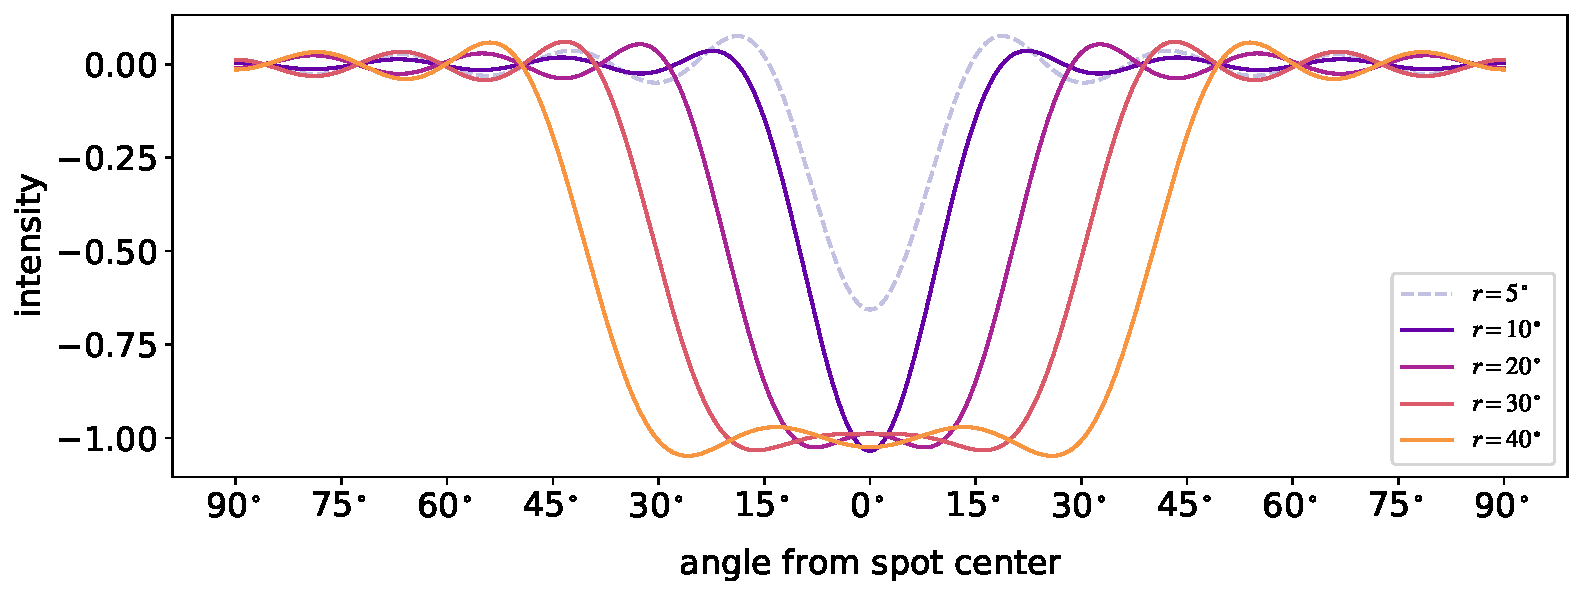
\includegraphics[width=\linewidth]{figures/spot_profile.pdf}
        \oscaption{spot_profile}{%
            Intensity profiles for spots with different
            radii $r$ computed at spherical harmonic
            degree $l_{\mathrm{max}} = \LMAX$.
            For $r \gtrsim 10^\circ$, the spherical harmonic expansion
            captures the spot shape and intensity reasonably well,
            albeit with some ringing due to the truncated expansion.
            \label{fig:spot_profile}
        }
    \end{centering}
\end{figure}

Figure~\ref{fig:spot_profile} shows the intensity profile for spots of
different radii expanded to spherical harmonic degree $l_{\mathrm{max}} = \LMAX$.
% computed from
% %
% \begin{align}
%     \mathbf{b'}(r) & = \mathbf{B}
%     \mathbf{B}^+ \, \mathbf{b}(r) \quad.
% \end{align}
%
The average intensity
within the spots is close to $-1$ and the half-widths at half-minimum are
equal to the spot radii, as expected.
The effect of ringing due to the truncated spherical harmonic expansion is
evident, although it is strongly suppressed compared to an expansion
without the smoothing term (i.e., $\sigma = \infty$). However, for
$r \lesssim 10^\circ$, an expansion to $l_{\mathrm{max}} = \LMAX$ is
insufficient to correctly model the spot, as can be seen from the
$r = 5^\circ$ profile (dashed curve). Expansions to higher spherical harmonic
degree allow one to model spots with radii smaller than $10^\circ$, although
at increased computational cost and potential numerical stability issues;
we discuss this point at length in \S\ref{sec:tiny-spots}.


\subsection{Probability density function}
%
For simplicity, we will adopt a uniform probability distribution for the
spot radius, characterized by a mean radius $r_0$ and a half-width $\Delta$:
%
\begin{align}
    p(r \, \big| \, \pmb{\theta}_{r})
    &=
    \begin{cases}
        \frac{1}{2\Delta} & r_0 - \Delta \leq r \leq r_0 + \Delta
        \\
        0 & \mathrm{otherwise}
        \quad,
    \end{cases}
\end{align}
%
where the hyperparameters of the distribution are
%
\begin{align}
    \pmb{\theta}_r = \left(
    r_0 \, \, \, \,
    \Delta \right)^\top
    \quad.
\end{align}
%
As we argue in the text, in practice it is often difficult to constrain the 
moments of the radius distribution above the first (the mean). It is 
therefore useful to also consider the limiting case of the radius distribution
as $\Delta \rightarrow 0$, in which case the PDF becomes
%
\begin{align}
    p(r \, \big| \, \pmb{\theta}_{r}, \Delta = 0)
    &=
    \delta(r - r_0)
    \quad,
\end{align}
%
where $\delta$ is the delta function.
%

\subsection{First moment}
%
The first moment of the radius distribution is (Equation~\ref{eq:e1})
%
\begin{align}
    \mathbf{e}_r
     & \equiv
    \int
    \mathbf{s}(r) \,
    p(r \, \big| \, \pmb{\theta}_{r}) \,
    \mathrm{d}r
    \nonumber \\
    &=
    \frac{1}{2\Delta}
    \int_{r_0 - \Delta}^{r_0 + \Delta}
    \mathbf{s}(r) \,
    \mathrm{d}r
    \quad.
\end{align}
%
Using the equations from the previous section, its components may be written
%
\begin{align}
    (e_r)^l_m
    &=
    \frac{\delta_{m,0}}{2\Delta}
    \int_{r_0 - \Delta}^{r_0 + \Delta}
    \tilde{s}_{l}(r) \,
    \mathrm{d}r
    \nonumber \\
    &=
    \frac{\delta_{m,0}}{2\Delta}
    \sum_{k=0}^{K-1} B^+_{l,k}
    \int_{r_0 - \Delta}^{r_0 + \Delta}
    b_{k}(r)
    \mathrm{d}r
    \nonumber \\
    &=
    \frac{\delta_{m,0} s}{2\Delta}
    \sum_{k=0}^{K-1} B^+_{l,k}
    \ln 
    \left(
        \frac{
            1+\exp\left(\frac{r -\Delta -\vartheta_k}{s}\right)
        }
        {
            1+\exp\left(\frac{r + \Delta -\vartheta_k}{s}\right)
        }
    \right)
    \quad.
\end{align}
%
In the limit $\Delta \rightarrow 0$,
%
\begin{align}
    \lim_{\Delta \rightarrow 0}
    \mathbf{e}_r
    &=
    \mathbf{B}^+ \mathbf{b}(r)
    \quad.
\end{align}
%

\subsection{Second moment}
%
The second moment of the radius distribution is (Equation~\ref{eq:E1})
%
\begin{align}
    \mathbf{E}_r
     & \equiv
    \int
    \mathbf{s}(r) \,
    \mathbf{s}^\top(r) \,
    p(r \, \big| \, \pmb{\theta}_{r}) \,
    \mathrm{d}r
    \nonumber \\
    &=
    \frac{1}{2\Delta}
    \int_{r_0 - \Delta}^{r_0 + \Delta}
    \mathbf{s}(r) \,
    \mathbf{s}^\top(r) \,
    \mathrm{d}r
    \quad.
\end{align}
%
As before, its components may be written
%
%
\begin{align}
    (E_r)^{l,l'}_{m,m'}
    &=
    \frac{\delta_{m,0}\delta_{m',0}}{2\Delta}
    \int_{r_0 - \Delta}^{r_0 + \Delta}
    \tilde{s}^l_{m}(r) \,
    \tilde{s}^{l'}_{m'}(r) \,
    \mathrm{d}r
    \nonumber \\
    &=
    \frac{\delta_{m,0}\delta_{m',0}}{2\Delta}
    \sum_{k=0}^{K-1} B^+_{l,k}
    \sum_{k'=0}^{K-1} B^+_{l',k'}
    \int_{r_0 - \Delta}^{r_0 + \Delta}
    b_{k}(r)
    b_{k'}(r)
    \mathrm{d}r
    \nonumber \\
    &= 
    \frac{\delta_{m,0}\delta_{m',0}s}{2\Delta}
    \sum_{k=0}^{K-1} B^+_{l,k}
    \sum_{k'=0}^{K-1} B^+_{l',k'}
    C_{k,k'}(r)
    \quad,
\end{align}
%
where
%
\begin{align}
    C_{k,k'}(r)
    &\equiv
    \frac{
        \exp\left(\frac{\vartheta_{k} - \vartheta_{k'}}{s}\right)
        \ln 
        \left(
            \frac{
                1+\exp\left(\frac{r -\Delta -\vartheta_{k}}{s}\right)
            }
            {
                1+\exp\left(\frac{r + \Delta -\vartheta_{k}}{s}\right)
            }
        \right)
        -
        \ln 
        \left(
            \frac{
                1+\exp\left(\frac{r -\Delta -\vartheta_{k'}}{s}\right)
            }
            {
                1+\exp\left(\frac{r + \Delta -\vartheta_{k'}}{s}\right)
            }
        \right)
    }{
        1
        -
        \exp\left(\frac{\vartheta_{k} - \vartheta_{k'}}{s}\right)
    }
    \quad.
\end{align}
%
In the limit $\Delta \rightarrow 0$,
%
\begin{align}
    \lim_{\Delta \rightarrow 0}
    \mathbf{E}_r
    &=
    \mathbf{B}^+ \mathbf{b}(r) \mathbf{b}^\top(r) {\mathbf{B}^+}^\top
    \quad.
\end{align}
%

\section{The Latitude and Longitude Integrals}
\label{sec:lat-lon}
%
Our goal in this section is to compute the first and second moments
of the latitude ($\mathbf{e}_\phi$, $\mathbf{E}_\phi$)
and longitude ($\mathbf{e}_\lambda$, $\mathbf{E}_\lambda$) distributions
(Equations \ref{eq:e2}, \ref{eq:e3}, \ref{eq:E2}, and \ref{eq:E3},
respectively). These involve integrals over the terms in the Wigner
rotation matrix for spherical harmonics, which we discuss below.

\subsection{Rotation matrices}
%
The Wigner rotation matrix for real spherical harmonics up to degree $l_{\mathrm{max}}$
may be written as the block-diagonal matrix
%
\begin{align}
    \setstackgap{L}{1.25\baselineskip}
    \fixTABwidth{T}
    \mathbf{R} =
    \parenMatrixstack{
    \quad\quad \, \mathbf{R}^0 \, \quad\quad
     &              &              &        &                               \\
     & \mathbf{R}^1 &              &        &                               \\
     &              & \mathbf{R}^2 &        &                               \\
     &              &              & \ddots &                               \\
     &              &              &        & \mathbf{R}^{l_{\mathrm{max}}}
    }\quad,
\end{align}
%
where
%
\begin{align}
    \mathbf{R}^l = {\mathbf{U}^l}^{-1} \mathbf{D}^l \mathbf{U}^l
\end{align}
%
is the Wigner rotation matrix for a single spherical harmonic degree,
%
\begin{align}
    \label{eq:U}
    \setstackgap{L}{1.25\baselineskip}
    \fixTABwidth{T}
    \mathbf{U}^l =
    \frac{1}{\sqrt{2}}
    \parenMatrixstack{
        \quad\quad\, \ddots \, \quad\quad\quad\quad
           &       &        &       &          &    &   &    & \Ddots \\
           & \imag &        &       &          &    &   & 1  &        \\
           &       & \imag  &       &          &    & 1 &    &        \\
           &       &        & \imag &          & 1  &   &    &        \\
           &       &        &       & \sqrt{2} &    &   &    &        \\
           &       &        & \imag &          & -1 &   &    &        \\
           &       & -\imag &       &          &    & 1 &    &        \\
           & \imag &        &       &          &    &   & -1 &        \\
    \Ddots &       &        &       &          &    &   &    & \ddots
    }
\end{align}
%
describes the transformation from complex to real spherical harmonics,
and $\mathbf{D}$ is the Wigner matrix for complex spherical harmonics,
whose terms are given by the expression
%
\begin{align}
    D_{m,m'}^l(\alpha, \beta, \gamma) = \mathrm{e}^{-\imag m' \alpha}
    d_{m,m'}^l(\beta) \mathrm{e}^{-\imag m \gamma}
\end{align}
%
where $\alpha$, $\beta$, and $\gamma$ are the Euler angles describing
the rotation in the
$\hat{\mathbf{z}}{-}\hat{\mathbf{y}}{-}\hat{\mathbf{z}}$ convention
and $\imag$ is the imaginary unit. The terms of the $d$-matrix
depend on powers of $\sin\left(\nicefrac{\beta}{2}\right)$
and $\cos\left(\nicefrac{\beta}{2}\right)$
\citep[c.f. Equation C15 in][]{Luger2019}, but it is convenient to use
the half-angle formula to express these terms instead as
%
\begin{proof}{test_dlmmp}
    d_{m,m'}^l(\beta) =
    \sum\limits_{i=0}^{2l} c_{m,m',i}^{l}
    \mathrm{sgn}(\sin\beta)^{i}
    (1 - \cos\beta)^{\frac{2l - i}{2}}
    (1 + \cos\beta)^\frac{i}{2}
\end{proof}
%
where
%
\begin{proof}{test_dlmmp}
    c_{m,m',i}^{l} & =
    \resizebox{.75\hsize}{!}{$
            \begin{cases}
                \dfrac{
                \left(-1\right)^{\frac{2l + 3m + m' - i}{2}}
                \sqrt{\left(l - m\right)!
                    \left(l + m\right)!
                    \left(l - m'\right)!
                    \left(l + m'\right)!}
                }{
                2^l
                \left(\frac{i - m - m'}{2}\right)!
                \left(\frac{i + m + m'}{2}\right)!
                \left(\frac{2l - i - m + m'}{2}\right)!
                \left(\frac{2l - i + m - m'}{2}\right)!
                }
                %
                 & m - m' - i \,\, \mathrm{even}
                %
                \\[0.5em]
                0
                %
                 & m - m' - i \,\, \mathrm{odd}
            \end{cases}
        $}
\end{proof}
%

\subsection{Latitude}
%
The latitude integrals (Equations~\ref{eq:e2} and \ref{eq:E2}) involve
rotations by an angle $\phi$ about $\hat{\mathbf{x}}$, which
may be accomplished by choosing
Euler angles $\alpha = \nicefrac{\pi}{2}$, $\beta = \phi$, and
$\gamma = -\nicefrac{\pi}{2}$, such that
%
\begin{align}
    \mathbf{R}^l_{\hat{\mathbf{x}}}(\phi)
     & =
    {\mathbf{U}^l}^{-1} \mathbf{D}^l_{\hat{\mathbf{x}}}(\phi) \mathbf{U}^l
\end{align}
%
with
\begin{align}
    \mathbf{D}^l_{\hat{\mathbf{x}}}(\phi)
     & =
    \mathbf{D}^l\left(\frac{\pi}{2}, \phi, -\frac{\pi}{2}\right)
    \quad.
\end{align}
%
From the expressions above, it is clear that all terms in
$\mathbf{R}_{\hat{\mathbf{x}}}(\phi)$ are equal to (weighted) sums of powers
of $(1 \pm \cos\phi)$.
%
Since our goal is to compute integrals of these terms multiplied by
a probability density function, it is convenient to model
$\cos\phi$ as a Beta-distributed variable. As we will see, this
choice will allow us to
analytically compute the first two moments of the distribution of
$\phi$ conditioned on $\pmb{\theta}_\phi$.

%
The Beta distribution in $\cos\phi$ has hyperparameters
%
\begin{align}
    \pmb{\theta}_\phi = \left(
    \alpha \, \, \, \,
    \beta \right)^\top
\end{align}
%
and PDF given by
%
\begin{align}
    \label{eq:cosphi-pdf}
    p \big(\cos\phi \, \big| \, \pmb{\theta}_\phi \big)
     & =
    \dfrac{\Gamma(\alpha + \beta)}{\Gamma(\alpha)\Gamma(\beta)}
    (\cos\phi)^{\alpha - 1}
    (1 - \cos\phi)^{\beta - 1}
    \quad,
\end{align}
%
where $\Gamma$ is the Gamma function. The implied distribution for $\phi$
may be computed by a straightforward change of variable:
%
\begin{proof}{test_beta_transform}
    \label{eq:phi-pdf}
    p \big(\phi \, \big| \, \pmb{\theta}_\phi \big)
    & =
    \dfrac{\Gamma(\alpha + \beta)}{2\Gamma(\alpha)\Gamma(\beta)}
    \big|
    \sin\phi
    \big|
    (\cos\phi)^{\alpha - 1}
    (1 - \cos\phi)^{\beta - 1}
    \quad,
\end{proof}
%
for $\phi \in \left[ -\frac{\pi}{2}, \frac{\pi}{2} \right]$.

\subsubsection{First moment}
%
Since the Wigner matrices are block diagonal, we may evaluate the moments of the
distribution one spherical harmonic degree at a time. To that end, let us
write the first moment integral as
%
\begin{proof}{test_ephi}
    \mathbf{e}_\phi
    & \equiv
    \int
    \mathbf{R}_{\hat{\mathbf{x}}}(\phi) \,
    \mathbf{e}_r \,
    p(\phi \, \big| \, \pmb{\theta}_{\phi}) \,
    \mathrm{d}\phi
    \nonumber
    \\
    %
    & =
    %
    \left(
    \mathbf{e}_\phi^0
    \,\,\,
    \mathbf{e}_\phi^1
    \,\,\,
    \mathbf{e}_\phi^2
    \,\,\,
    \cdots
    \,\,\,
    \mathbf{e}_\phi^{l_{\mathrm{max}}}
    \right)^\top
    \quad,
\end{proof}
%
where
%
\begin{proof}{test_ephi}
    \mathbf{e}_\phi^l
    & =
    \int
    \mathbf{R}^l_{\hat{\mathbf{x}}}(\phi) \,
    \mathbf{e}^l_r \,
    p(\phi \, \big| \, \pmb{\theta}_{\phi}) \,
    \mathrm{d}\phi
    \nonumber \\
    %
    & =
    %
    {\mathbf{U}^l}^{-1}
    \mathbf{p}^l
    \quad,
\end{proof}
%
and we define
%
\begin{align}
    \label{eq:plphi}
    \mathbf{p}^l_\phi
     & \equiv
    \int
    \mathbf{D}^l_{\hat{\mathbf{x}}}(\phi) \,
    \bar{\mathbf{e}}^l_r \,
    p(\phi \, \big| \, \pmb{\theta}_{\phi}) \,
    \mathrm{d}\phi
    \\
    \bar{\mathbf{e}}^l_r
     & \equiv
    \mathbf{U}^l
    \mathbf{e}^l_r
    \quad.
\end{align}
%
The integral $\mathbf{p}^l_\phi$ defined above has a closed-form solution.
To show this, we write the terms of $\mathbf{p}^l_\phi$ as
%
\begin{align}
    {p^l_\phi}_m
     & =
    \int
    \sum\limits_{\mu=-l}^l
    {D^l_{\hat{\mathbf{x}}}}_{m,\mu}(\phi) \,
    {\bar{e}^l}{{}_r}_{\mu} \,
    p(\phi \, \big| \, \pmb{\theta}_{\phi}) \,
    \mathrm{d}\phi
    %
    \nonumber \\[0.5em]
    %
     & =
    \dfrac{\Gamma(\alpha + \beta)}{\Gamma(\alpha)\Gamma(\beta)}
    \sum\limits_{\mu=-l}^l
    {\bar{e}^l}{{}_r}_{\mu}
    \mathrm{e}^{\frac{\imag \pi}{2}(m - \mu)}
    \sum\limits_{i=0}^{2l} c_{m,\mu,i}^{l}
    \,
    {q^l_\phi}_i(\pmb{\theta}_{\phi})
    \quad,
\end{align}
%
where
%
\begin{proof}{test_qlphii}
    {q^l_\phi}_i(\pmb{\theta}_{\phi})
    & \equiv
    \frac{1}{2}
    \int_{-\frac{\pi}{2}}^{\frac{\pi}{2}}
    %
    \mathrm{sgn}(\sin\phi)^{i}
    \big| \sin\phi \big|
    (\cos\phi)^{\alpha - 1}
    (1 - \cos\phi)^{l + \beta - \frac{i}{2} - 1}
    (1 + \cos\phi)^\frac{i}{2}
    %
    \,
    \mathrm{d}\phi
    \nonumber \\[0.5em]
    %
    & =
    %
    \begin{cases}
        \displaystyle\int_{0}^{1}
        %
        x^{\alpha - 1}
        (1 - x)^{l + \beta - \frac{i}{2} - 1 }
        (1 + x)^\frac{i}{2}
        %
        \,
        \mathrm{d}x
        %
         & i \,\, \mathrm{even}
        %
        \\
        %
        0
        %
         & i \,\, \mathrm{odd} \quad,
    \end{cases}
\end{proof}
%
and in the last line we made use of the transformation $x = \cos\phi$.
%
The integral in the expression above has a closed-form solution in terms
of the hypergeometric function $_2F_1$:
%
\begin{proof}{test_qlphii}
    %
    \label{eq:qlphii}
    {q^l_\phi}_i(\pmb{\theta}_{\phi})
    & =
    \resizebox{.75\hsize}{!}{$
            \begin{cases}
                \dfrac{\Gamma(\alpha)\Gamma(l + \beta - \frac{i}{2})}{\Gamma(l + \alpha + \beta - \frac{i}{2})}
                \,
                _2F_1\Big(
                -\frac{i}{2},
                \alpha;
                l + \alpha + \beta - \frac{i}{2};
                -1
                \Big)
                %
                 & i \,\, \mathrm{even}
                %
                \\
                %
                0
                %
                 & i \,\, \mathrm{odd} \quad.
            \end{cases}
        $}
\end{proof}
%
In order to compute the integral $\mathbf{e}_\phi$
(Equation~\ref{eq:e2}) we must evaluate Equation~(\ref{eq:qlphii})
for all $0 \leq l \leq l_{\mathrm{max}}$, $0 \leq i \leq 2l$,
which can be done efficiently via upward recursion relations for both
the gamma function and the hypergeometric function.

\subsubsection{Second moment}
%
Similarly as before, let us write the second moment integral as
%
\begin{proof}{}
    \mathbf{E}_\phi
    & \equiv
    \int
    \mathbf{R}_{\hat{\mathbf{x}}}(\phi) \,
    \mathbf{E}_r \,
    \mathbf{E}_r^\top \,
    \mathbf{R}_{\hat{\mathbf{x}}}^\top(\phi) \,
    p(\phi \, \big| \, \pmb{\theta}_{\phi}) \,
    \mathrm{d}\phi
    \nonumber
    \\
    %
    & =
    %
    \setstackgap{L}{1.25\baselineskip}
    \fixTABwidth{T}
    \parenMatrixstack{
    \mathbf{E}_\phi^{0,0} & \mathbf{E}_\phi^{0,1} & \mathbf{E}_\phi^{0,2} & \cdots & \mathbf{E}_\phi^{0,l_{\mathrm{max}}} \\
    \mathbf{E}_\phi^{1,0} & \mathbf{E}_\phi^{1,1} & \mathbf{E}_\phi^{1,2} & \cdots & \mathbf{E}_\phi^{1,l_{\mathrm{max}}} \\
    \mathbf{E}_\phi^{2,0} & \mathbf{E}_\phi^{2,1} & \mathbf{E}_\phi^{2,2} & \cdots & \mathbf{E}_\phi^{2,l_{\mathrm{max}}} \\
    \vdots & \vdots & \vdots & \ddots & \vdots \\
    \mathbf{E}_\phi^{l_{\mathrm{max}},0} & \mathbf{E}_\phi^{l_{\mathrm{max}},1} & \mathbf{E}_\phi^{l_{\mathrm{max}},2} & \cdots & \mathbf{E}_\phi^{l_{\mathrm{max}},l_{\mathrm{max}}}
    }
    \quad,
\end{proof}
%
where
%
\begin{proof}{}
    \mathbf{E}_\phi^{l,l'}
    & =
    \int
    \mathbf{R}^l_{\hat{\mathbf{x}}}(\phi) \,
    \mathbf{E}^l_r \,
    {\mathbf{E}^l_r}^\top \,
    {\mathbf{R}^{l'}_{\hat{\mathbf{x}}}}^\top(\phi) \,
    p(\phi \, \big| \, \pmb{\theta}_{\phi}) \,
    \mathrm{d}\phi
    \nonumber \\
    %
    & =
    %
    {\mathbf{U}^l}^{-1}
    \mathbf{P}^l_\phi
    {{\mathbf{U}^l}^{-1}}^\top
\end{proof}
%
and we define
%
\begin{align}
    \label{eq:Plphi}
    \mathbf{P}^l_\phi
     & \equiv
    \int
    \mathbf{D}^l_{\hat{\mathbf{x}}}(\phi) \,
    \bar{\mathbf{E}}^l_r \,
    {\mathbf{D}^l_{\hat{\mathbf{x}}}}^\top(\phi) \,
    p(\phi \, \big| \, \pmb{\theta}_{\phi}) \,
    \mathrm{d}\phi
    \\
    \bar{\mathbf{E}}^l_r
     & \equiv
    \mathbf{U}^l
    \mathbf{E}^l_r
    {\mathbf{E}^l_r}^\top
    {\mathbf{U}^l}^\top
    \quad.
\end{align}
%
As before, we may express the solution to the integral $\mathbf{P}^l_\phi$ in
closed form. Let us write the terms of $\mathbf{P}^l_\phi$ as
%
\begin{align}
    {P^l_\phi}_{m,m'}
     & =
    \int
    \sum\limits_{\mu=-l}^l
    \sum\limits_{\nu=-l}^l
    {D^l_{\hat{\mathbf{x}}}}_{m,\mu}(\phi) \,
    {\bar{E}^l}{{}_r}_{\mu,\nu} \,
    {D^l_{\hat{\mathbf{x}}}}_{\nu,m'}(\phi) \,
    p(\phi \, \big| \, \pmb{\theta}_{\phi}) \,
    \mathrm{d}\phi
    %
    \nonumber \\[0.5em]
    %
     & =
    \resizebox{.75\hsize}{!}{$
        \dfrac{\Gamma(\alpha + \beta)}{\Gamma(\alpha)\Gamma(\beta)}
        \sum\limits_{\mu=-l}^l
        \sum\limits_{\nu=-l}^l
        {\bar{E}^l}{{}_r}_{\mu,\nu}
        \mathrm{e}^{\frac{\imag \pi}{2}(m - \mu + \nu - m')}
        \sum\limits_{i=0}^{2l}
        \sum\limits_{j=0}^{2l}
        c_{m,\mu,i}^{l}
        c_{\nu,m',j}^{l}
        \,
        {Q^l_\phi}_{i,j}(\pmb{\theta}_{\phi})
    $}
    \quad,
\end{align}
%
where, similarly to before,
%
\begin{proof}{}
    {Q^l_\phi}_{i,j}(\pmb{\theta}_{\phi})
    & \equiv
    \frac{1}{2}
    \int_{-\frac{\pi}{2}}^{\frac{\pi}{2}}
    %
    \mathrm{sgn}(\sin\phi)^{i+j}
    \big| \sin\phi \big|
    (\cos\phi)^{\alpha - 1}
    (1 - \cos\phi)^{2l + \beta - \frac{i+j}{2} - 1}
    (1 + \cos\phi)^\frac{i+j}{2}
    %
    \,
    \mathrm{d}\phi
    \nonumber \\[0.5em]
    %
    & =
    %
    \begin{cases}
        \displaystyle\int_{0}^{1}
        %
        x^{\alpha - 1}
        (1 - x)^{2l + \beta - \frac{i+j}{2} - 1 }
        (1 + x)^\frac{i+j}{2}
        %
        \,
        \mathrm{d}x
        %
         & i+j \,\, \mathrm{even}
        %
        \\
        %
        0
        %
         & i+j \,\, \mathrm{odd} \quad.
    \end{cases}
\end{proof}
%
We may again express this integral in closed form:
%
\begin{proof}{}
    %
    \label{eq:Qlphiij}
    {Q^l_\phi}_{i,j}(\pmb{\theta}_{\phi})
    & =
    \resizebox{.75\hsize}{!}{$
            \begin{cases}
                \dfrac{\Gamma(\alpha)\Gamma(2l + \beta - \frac{i+j}{2})}{\Gamma(2l + \alpha + \beta - \frac{i+j}{2})}
                \,
                _2F_1\Big(
                -\frac{i+j}{2},
                \alpha;
                2l + \alpha + \beta - \frac{i+j}{2};
                -1
                \Big)
                %
                 & i+j \,\, \mathrm{even}
                %
                \\
                %
                0
                %
                 & i+j \,\, \mathrm{odd} \quad.
            \end{cases}
        $}
\end{proof}
%
As before, this integral may be evaluated recursively to efficiently compute all
of the terms in $\mathbf{E}_\phi$.

\subsection{Longitude}
%
The longitude integrals (Equations~\ref{eq:e3} and \ref{eq:E3}) involve
rotations by an angle $\lambda$ about $\hat{\mathbf{y}}$, which
may be accomplished by choosing
Euler angles $\alpha = 0$, $\beta = \lambda$, and
$\gamma = 0$, such that
%
\begin{align}
    \mathbf{R}^l_{\hat{\mathbf{y}}}(\lambda)
     & =
    {\mathbf{U}^l}^{-1} \mathbf{D}^l_{\hat{\mathbf{y}}}(\lambda) \mathbf{U}^l
\end{align}
%
with
\begin{align}
    \mathbf{D}^l_{\hat{\mathbf{y}}}(\lambda)
     & =
    \mathbf{D}^l\left(0, \lambda, 0\right)
    \quad.
\end{align}
%
Since we expect the longitudinal distribution of features on the surfaces
of stars to be (on average) isotropic, we will place a uniform prior on
$\lambda \in [-\pi, \pi)$:
%
\begin{align}
    p(\lambda \big| \pmb{\theta}_\lambda)
     & =
    \begin{cases}
        \frac{1}{2\pi} & -\pi \leq \lambda < \pi
        \\
        0              & \mathrm{otherwise} \quad.
    \end{cases}
\end{align}
%
We therefore have no hyperparameters
controlling the longitudinal distribution, i.e.,
%
\begin{align}
    \pmb{\theta}_\lambda = \left( \,\,\, \right)
    \quad.
\end{align}
%

\subsubsection{First moment}
%
As before, we will solve for the terms of the moment integrals one
spherical harmonic degree at a time:
%
\begin{proof}{test_elam}
    \mathbf{e}_\lambda
    & \equiv
    \int
    \mathbf{R}_{\hat{\mathbf{y}}}(\lambda) \,
    \mathbf{e}_\phi \,
    p(\lambda \, \big| \, \pmb{\theta}_{\lambda}) \,
    \mathrm{d}\lambda
    \nonumber
    \\
    %
    & =
    %
    \left(
    \mathbf{e}_\lambda^0
    \,\,\,
    \mathbf{e}_\lambda^1
    \,\,\,
    \mathbf{e}_\lambda^2
    \,\,\,
    \cdots
    \,\,\,
    \mathbf{e}_\lambda^{l_{\mathrm{max}}}
    \right)^\top
    \quad,
\end{proof}
%
where
%
\begin{proof}{test_elam}
    \mathbf{e}_\lambda^l
    & =
    \int
    \mathbf{R}^l_{\hat{\mathbf{y}}}(\lambda) \,
    \mathbf{e}^l_\phi \,
    p(\lambda \, \big| \, \pmb{\theta}_{\lambda}) \,
    \mathrm{d}\lambda
    \nonumber \\
    %
    & =
    %
    {\mathbf{U}^l}^{-1}
    \mathbf{p}^l_\lambda
    \quad,
\end{proof}
%
and we define
%
\begin{align}
    \label{eq:pllam}
    \mathbf{p}^l_\lambda
     & \equiv
    \int
    \mathbf{D}^l_{\hat{\mathbf{x}}}(\lambda) \,
    \bar{\mathbf{e}}^l_\phi \,
    p(\lambda \, \big| \, \pmb{\theta}_{\lambda}) \,
    \mathrm{d}\lambda
    \\
    \bar{\mathbf{e}}^l_\phi
     & \equiv
    \mathbf{U}^l
    \mathbf{e}^l_\phi
    \quad.
\end{align}
%
The integral $\mathbf{p}^l_\lambda$ defined above has a closed-form solution.
To show this, we write the terms of $\mathbf{p}^l_\lambda$ as
%
\begin{align}
    {p^l_\lambda}_m
     & =
    \int
    \sum\limits_{\mu=-l}^l
    {D^l_{\hat{\mathbf{y}}}}_{m,\mu}(\lambda) \,
    {\bar{e}^l}{{}_\phi}_{\mu} \,
    p(\lambda \, \big| \, \pmb{\theta}_{\lambda}) \,
    \mathrm{d}\lambda
    %
    \nonumber \\[0.5em]
    %
     & =
    \sum\limits_{\mu=-l}^l
    {\bar{e}^l}{{}_\phi}_{\mu}
    \sum\limits_{i=0}^{2l} c_{m,\mu,i}^{l}
    \,
    {q^l_\lambda}_i
    \quad,
\end{align}
%
where
%
\begin{proof}{test_qllam}
    {q^l_\lambda}_i
    & \equiv
    \frac{1}{2\pi}
    \int_{-\pi}^{\pi}
    %
    \mathrm{sgn}(\sin\lambda)^{i}
    (1 - \cos\lambda)^{l - \frac{i}{2}}
    (1 + \cos\lambda)^\frac{i}{2}
    %
    \,
    \mathrm{d}\lambda
    \nonumber \\[0.5em]
    %
    & =
    %
    \begin{cases}
        \dfrac{2^l \Gamma \left(\frac{1+i}{2}\right)
            \Gamma \left(l+\frac{1-i}{2}\right)}{\pi  \Gamma (l+1)}
        %
         & i \,\, \mathrm{even}
        %
        \\
        %
        0
        %
         & i \,\, \mathrm{odd} \quad,
    \end{cases}
\end{proof}
%
whose terms may easily be computed by upward recursion.

\subsubsection{Second moment}
%
We write the second moment integral as
%
\begin{proof}{}
    \mathbf{E}_\lambda
    & \equiv
    \int
    \mathbf{R}_{\hat{\mathbf{y}}}(\lambda) \,
    \mathbf{E}_\phi \,
    \mathbf{E}_\phi^\top \,
    \mathbf{R}_{\hat{\mathbf{y}}}^\top(\lambda) \,
    p(\lambda \, \big| \, \pmb{\theta}_{\lambda}) \,
    \mathrm{d}\lambda
    \nonumber
    \\
    %
    & =
    %
    \setstackgap{L}{1.25\baselineskip}
    \fixTABwidth{T}
    \parenMatrixstack{
    \mathbf{E}_\lambda^{0,0} & \mathbf{E}_\lambda^{0,1} & \mathbf{E}_\lambda^{0,2} & \cdots & \mathbf{E}_\lambda^{0,l_{\mathrm{max}}} \\
    \mathbf{E}_\lambda^{1,0} & \mathbf{E}_\lambda^{1,1} & \mathbf{E}_\lambda^{1,2} & \cdots & \mathbf{E}_\lambda^{1,l_{\mathrm{max}}} \\
    \mathbf{E}_\lambda^{2,0} & \mathbf{E}_\lambda^{2,1} & \mathbf{E}_\lambda^{2,2} & \cdots & \mathbf{E}_\lambda^{2,l_{\mathrm{max}}} \\
    \vdots & \vdots & \vdots & \ddots & \vdots \\
    \mathbf{E}_\lambda^{l_{\mathrm{max}},0} & \mathbf{E}_\lambda^{l_{\mathrm{max}},1} & \mathbf{E}_\lambda^{l_{\mathrm{max}},2} & \cdots & \mathbf{E}_\lambda^{l_{\mathrm{max}},l_{\mathrm{max}}}
    }
    \quad,
\end{proof}
%
where
%
\begin{proof}{}
    \mathbf{E}_\lambda^{l,l'}
    & =
    \int
    \mathbf{R}^l_{\hat{\mathbf{y}}}(\lambda) \,
    \mathbf{E}^l_\phi \,
    {\mathbf{E}^l_\phi}^\top \,
    {\mathbf{R}^{l'}_{\hat{\mathbf{y}}}}^\top(\lambda) \,
    p(\lambda \, \big| \, \pmb{\theta}_{\lambda}) \,
    \mathrm{d}\lambda
    \nonumber \\
    %
    & =
    %
    {\mathbf{U}^l}^{-1}
    \mathbf{P}^l_\lambda
    {{\mathbf{U}^l}^{-1}}^\top
\end{proof}
%
and we define
%
\begin{align}
    \label{eq:Pllam}
    \mathbf{P}^l_\lambda
     & \equiv
    \int
    \mathbf{D}^l_{\hat{\mathbf{x}}}(\lambda) \,
    \bar{\mathbf{E}}^l_\phi \,
    {\mathbf{D}^l_{\hat{\mathbf{x}}}}^\top(\lambda) \,
    p(\lambda \, \big| \, \pmb{\theta}_{\lambda}) \,
    \mathrm{d}\lambda
    \\
    \bar{\mathbf{E}}^l_\phi
     & \equiv
    \mathbf{U}^l
    \mathbf{E}^l_\phi
    {\mathbf{E}^l_\phi}^\top
    {\mathbf{U}^l}^\top
    \quad.
\end{align}
%
We then express the terms of $\mathbf{P}^l_\lambda$ as
%
\begin{align}
    {P^l_\lambda}_{m,m'}
     & =
    \int
    \sum\limits_{\mu=-l}^l
    \sum\limits_{\nu=-l}^l
    {D^l_{\hat{\mathbf{x}}}}_{m,\mu}(\lambda) \,
    {\bar{E}^l}{{}_\phi}_{\mu,\nu} \,
    {D^l_{\hat{\mathbf{x}}}}_{\nu,m'}(\lambda) \,
    p(\lambda \, \big| \, \pmb{\theta}_{\lambda}) \,
    \mathrm{d}\lambda
    %
    \nonumber \\[0.5em]
    %
     & =
    \sum\limits_{\mu=-l}^l
    \sum\limits_{\nu=-l}^l
    {\bar{E}^l}{{}_\phi}_{\mu,\nu}
    \sum\limits_{i=0}^{2l}
    \sum\limits_{j=0}^{2l}
    c_{m,\mu,i}^{l}
    c_{\nu,m',j}^{l}
    \,
    {Q^l_\lambda}_{i,j}
    \quad,
\end{align}
%
where
%
\begin{proof}{}
    {Q^l_\lambda}_{i,j}
    & \equiv
    \frac{1}{2\pi}
    \int_{-\pi}^{\pi}
    %
    \mathrm{sgn}(\sin\lambda)^{i+j}
    (1 - \cos\lambda)^{2l - \frac{i+j}{2}}
    (1 + \cos\lambda)^\frac{i+j}{2}
    %
    \,
    \mathrm{d}\lambda
    \nonumber \\[0.5em]
    %
    & =
    %
    \begin{cases}
        \dfrac{2^{2l} \Gamma \left(\frac{1+i+j}{2}\right)
            \Gamma \left(2l+\frac{1-i-j}{2}\right)}{\pi  \Gamma (2l+1)}
        %
         & i+j \,\, \mathrm{even}
        %
        \\
        %
        0
        %
         & i+j \,\, \mathrm{odd} \quad,
    \end{cases}
\end{proof}
%
whose terms may again be computed by upward recursion.


\section{The Contrast Integral}
\label{sec:contrast}
%
\xxx{Coming soon.}

\bibliography{bib}
\end{document}